\newcounter{case}
\newcommand\case{\stepcounter{case}\arabic{case}}
\newenvironment{preface}{\clearpage\setlength{\topskip}{0pt}%
  \newgeometry{vmargin=0cm,ignoreheadfoot}%
  \thispagestyle{empty}%
  \vspace*{\fill}\nointerlineskip\small}%
  {\vspace*{\fill}\clearpage\restoregeometry}
\chapter{USER INTERFACE DESIGN}
\label{ch:interfaceDesign}%
\section{eMSP Application}

\begin{figure}[H]
    \begin{minipage}[t]{.45\textwidth} % not "0.5\textwidth"
    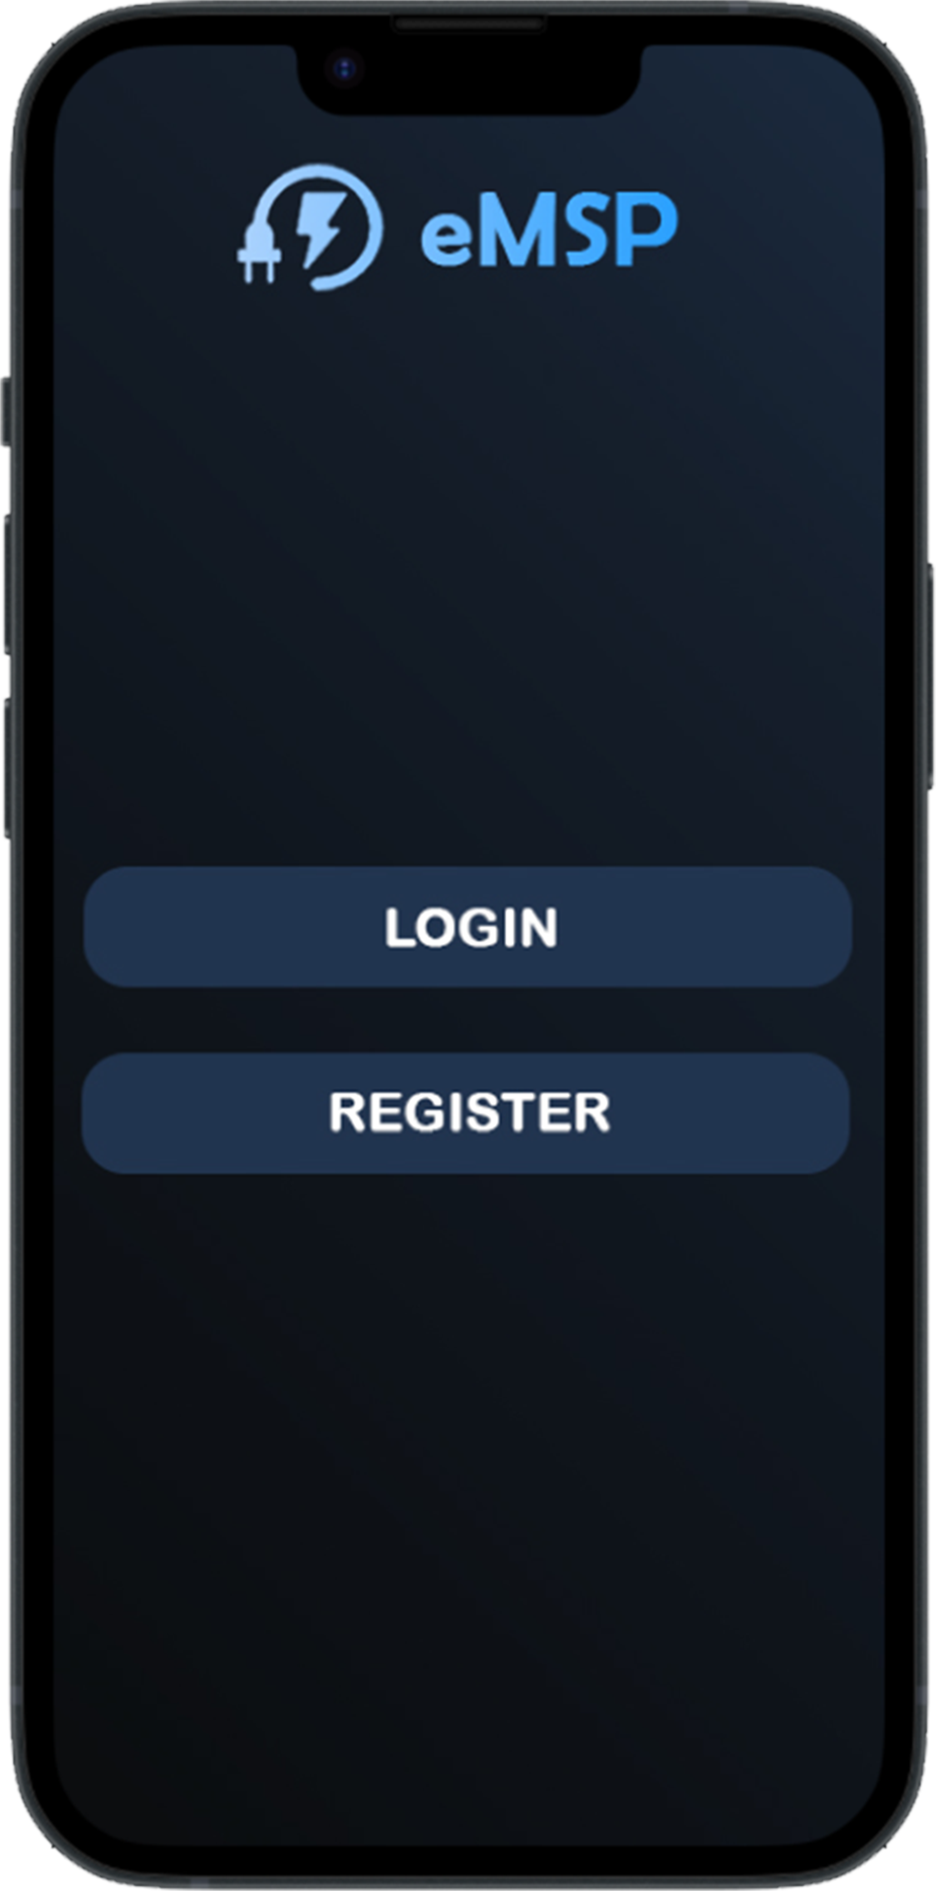
\includegraphics[width=\textwidth]{Mock/eMSP/MainPage}
    \caption{Main Page}
    \label{fig:MainPage}
\end{minipage}
\hfill
\begin{minipage}[t]{.45\textwidth}
    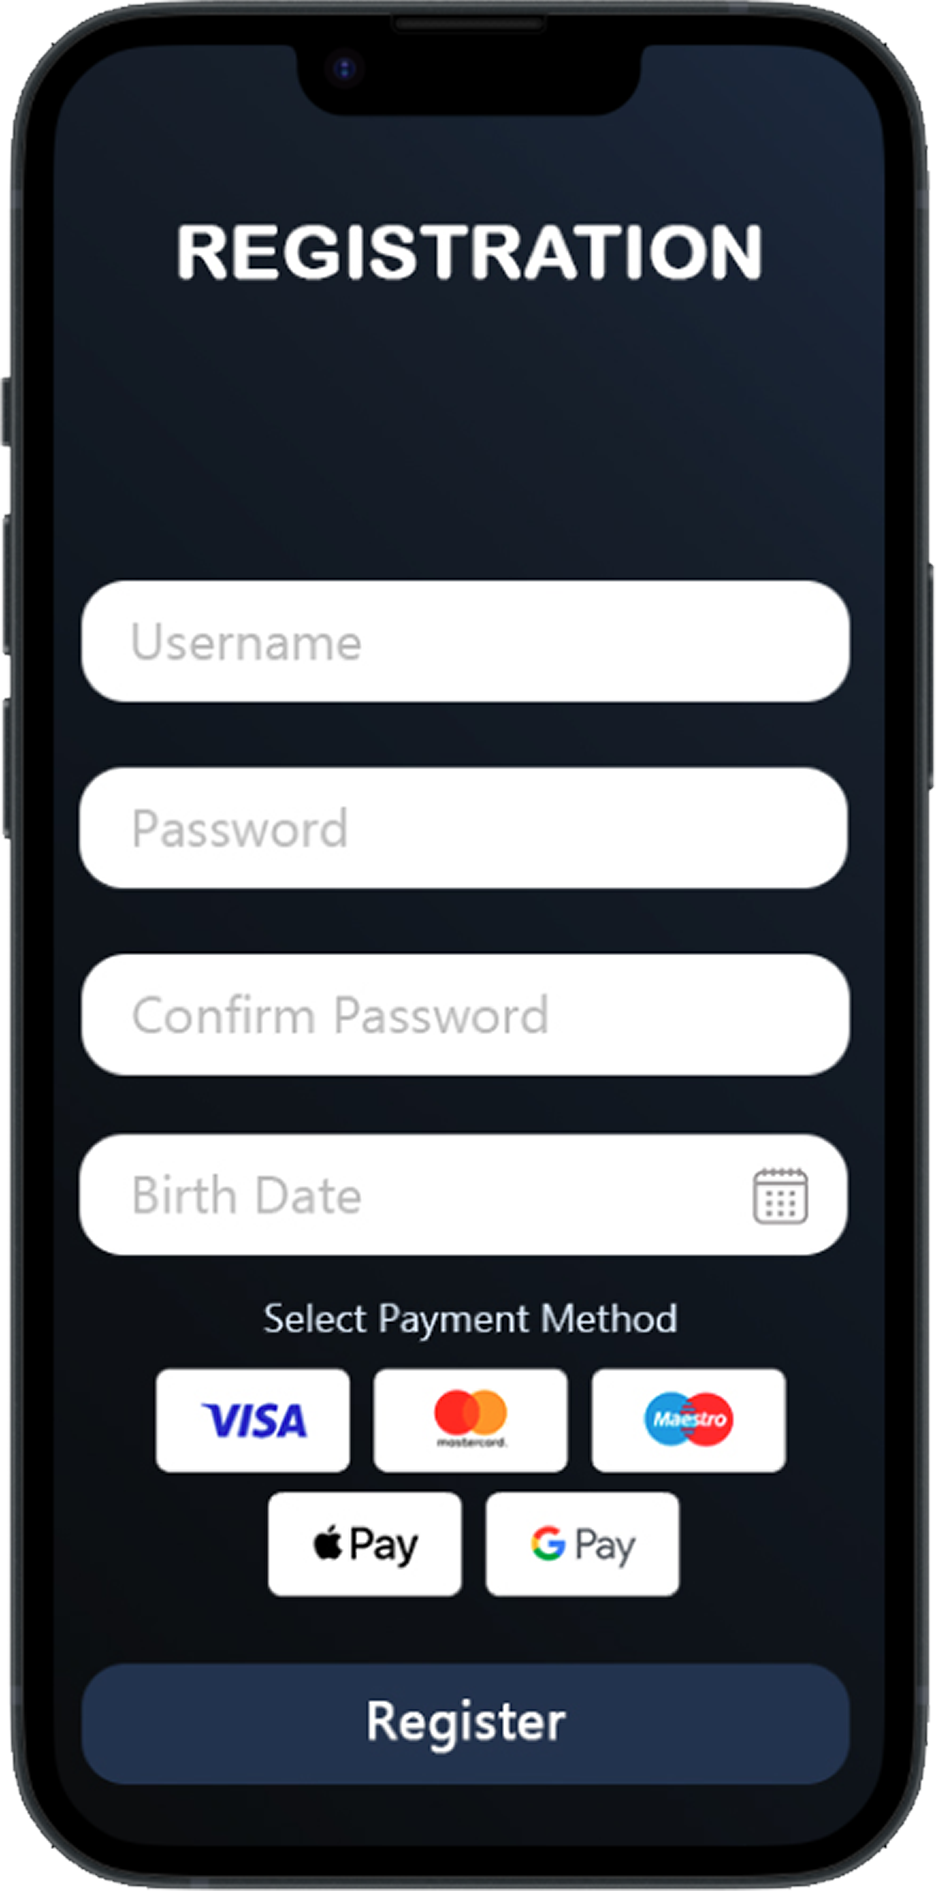
\includegraphics[width=\textwidth]{Mock/eMSP/Registration}
    \caption{Registration Page}
    \label{fig:Registration}
\end{minipage}
\end{figure}
These two mockups display the main page on the left, which has two buttons that redirect to the login and registration pages on the right. The registration page allows Unregistered Drivers to sign up for the eMSP by submitting their personal data and a payment method.
\begin{preface}
\begin{figure}[H]
    \begin{minipage}[t]{.45\textwidth} % not "0.5\textwidth"
    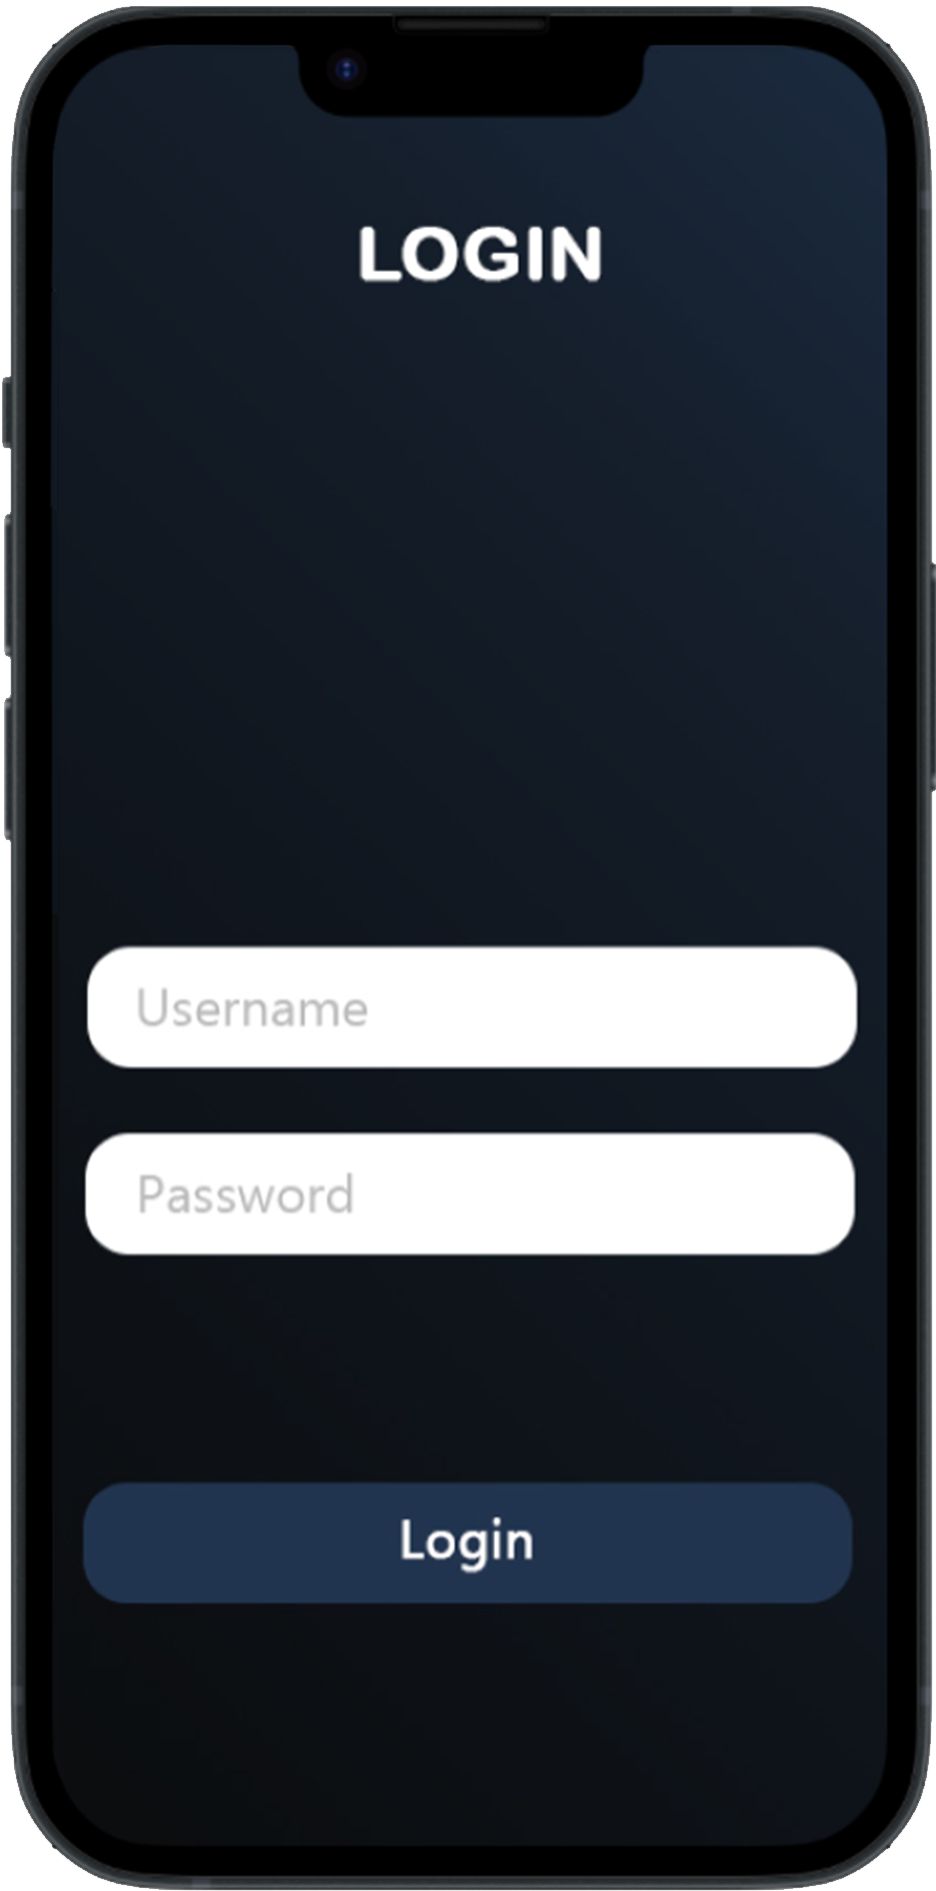
\includegraphics[width=\textwidth]{Mock/eMSP/eMSPLogin}
    \caption{Login Page}
    \label{fig:eMSPLogin}
\end{minipage}
\hfill
\begin{minipage}[t]{.45\textwidth}
    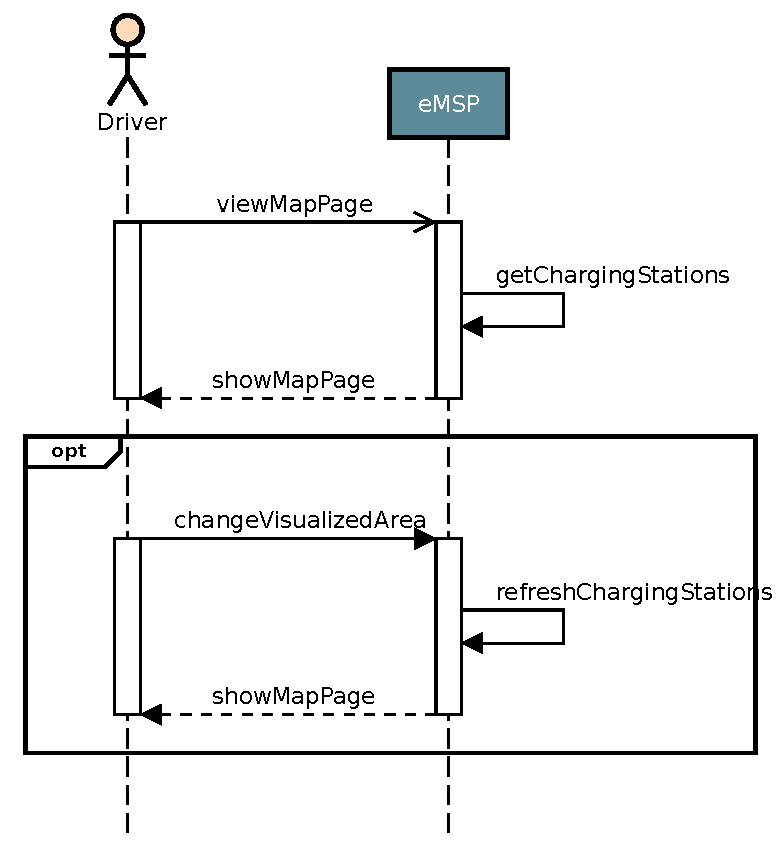
\includegraphics[width=\textwidth]{Mock/eMSP/Map}
    \caption{Map Page}
    \label{fig:Map}
\end{minipage}
\end{figure}
The image on the left depicts the login page for the Driver, while the image on the right shows the map page of the eMSP mobile application. This page allows the Driver to navigate the map, set filters, click on stations, and access his booking page.
\end{preface}
\begin{preface}
\begin{figure}[H]
    \begin{minipage}[t]{.45\textwidth} % not "0.5\textwidth"
    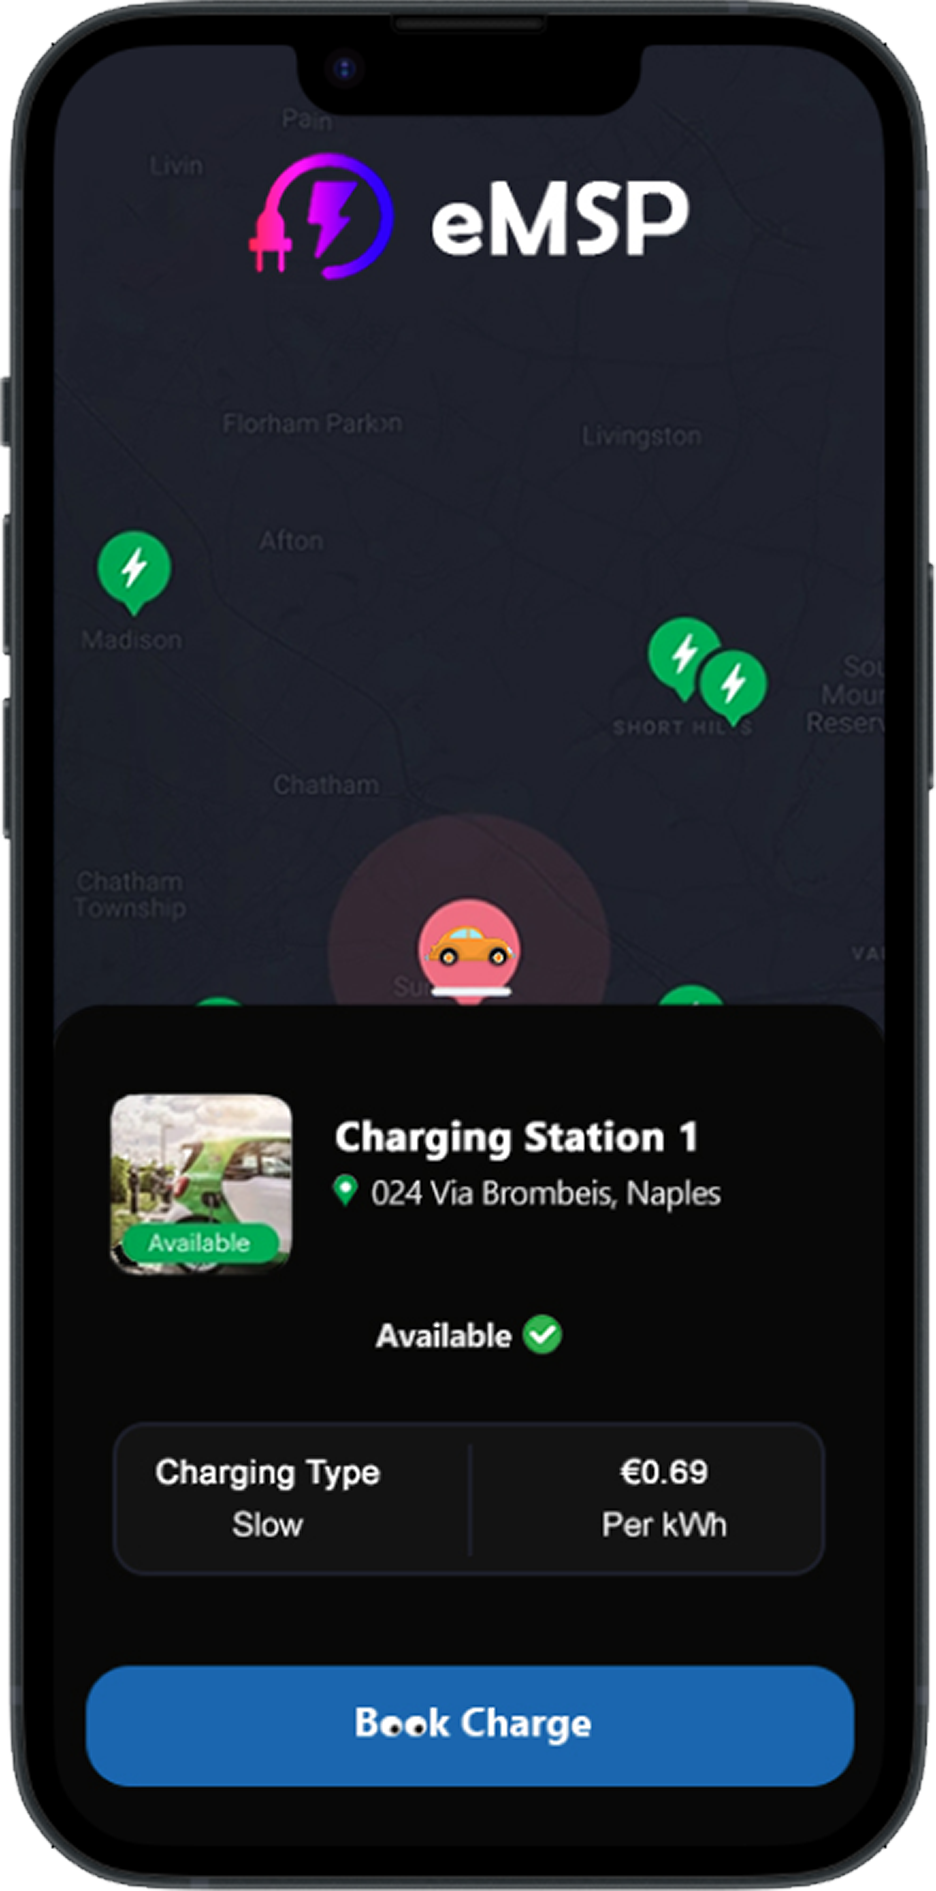
\includegraphics[width=\textwidth]{Mock/eMSP/StationInfo}
    \caption{Charging Station Info Page}
    \label{fig:StationInfo}
\end{minipage}
\hfill
\begin{minipage}[t]{.45\textwidth}
    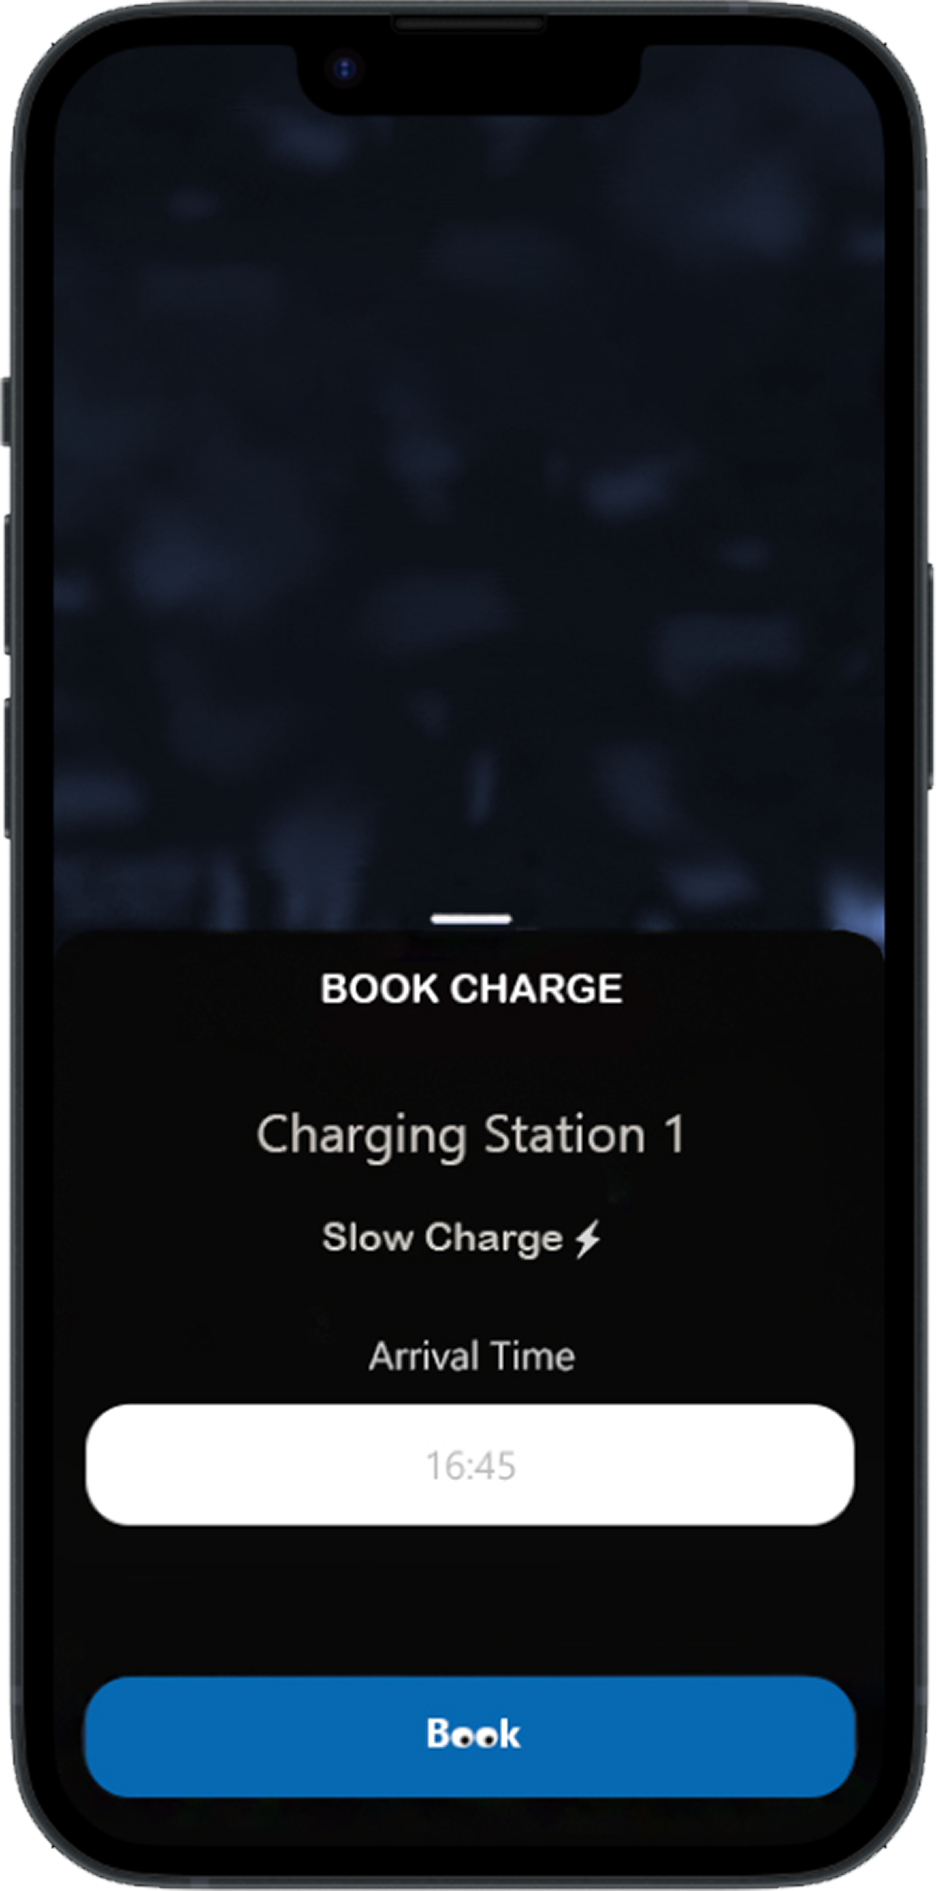
\includegraphics[width=\textwidth]{Mock/eMSP/BookCharge}
    \caption{Book Charge Page}
    \label{fig:BookCharge}
\end{minipage}
\end{figure}
These two mockups depict the charging station page on the left and the station's book charge page on the right. The charging station page allows the Driver to view information about the station, while the book charge page enables the Driver to book a charge for the selected charging type at the chosen arrival time.
\end{preface}
\begin{preface}
\begin{figure}[H]
    \begin{minipage}[t]{.45\textwidth} % not "0.5\textwidth"
    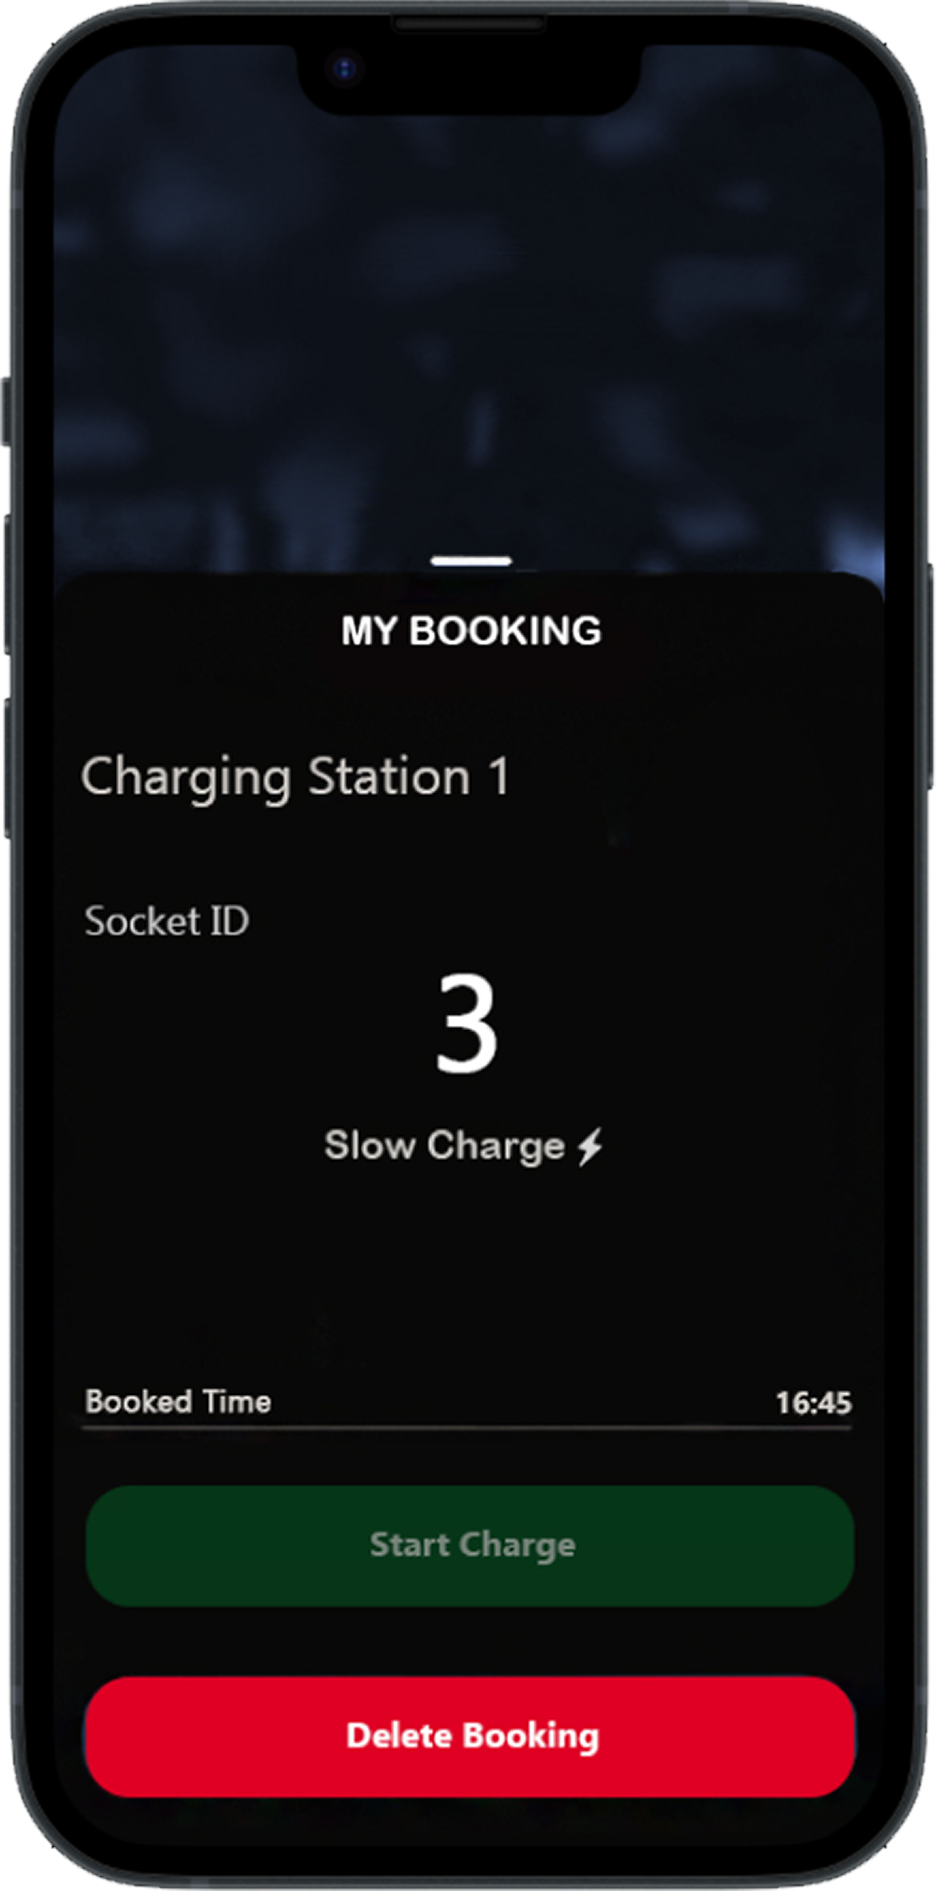
\includegraphics[width=\textwidth]{Mock/eMSP/MyBooking}
    \caption{My Booking Page}
    \label{fig:MyBooking}
\end{minipage}
\hfill
\begin{minipage}[t]{.45\textwidth}
    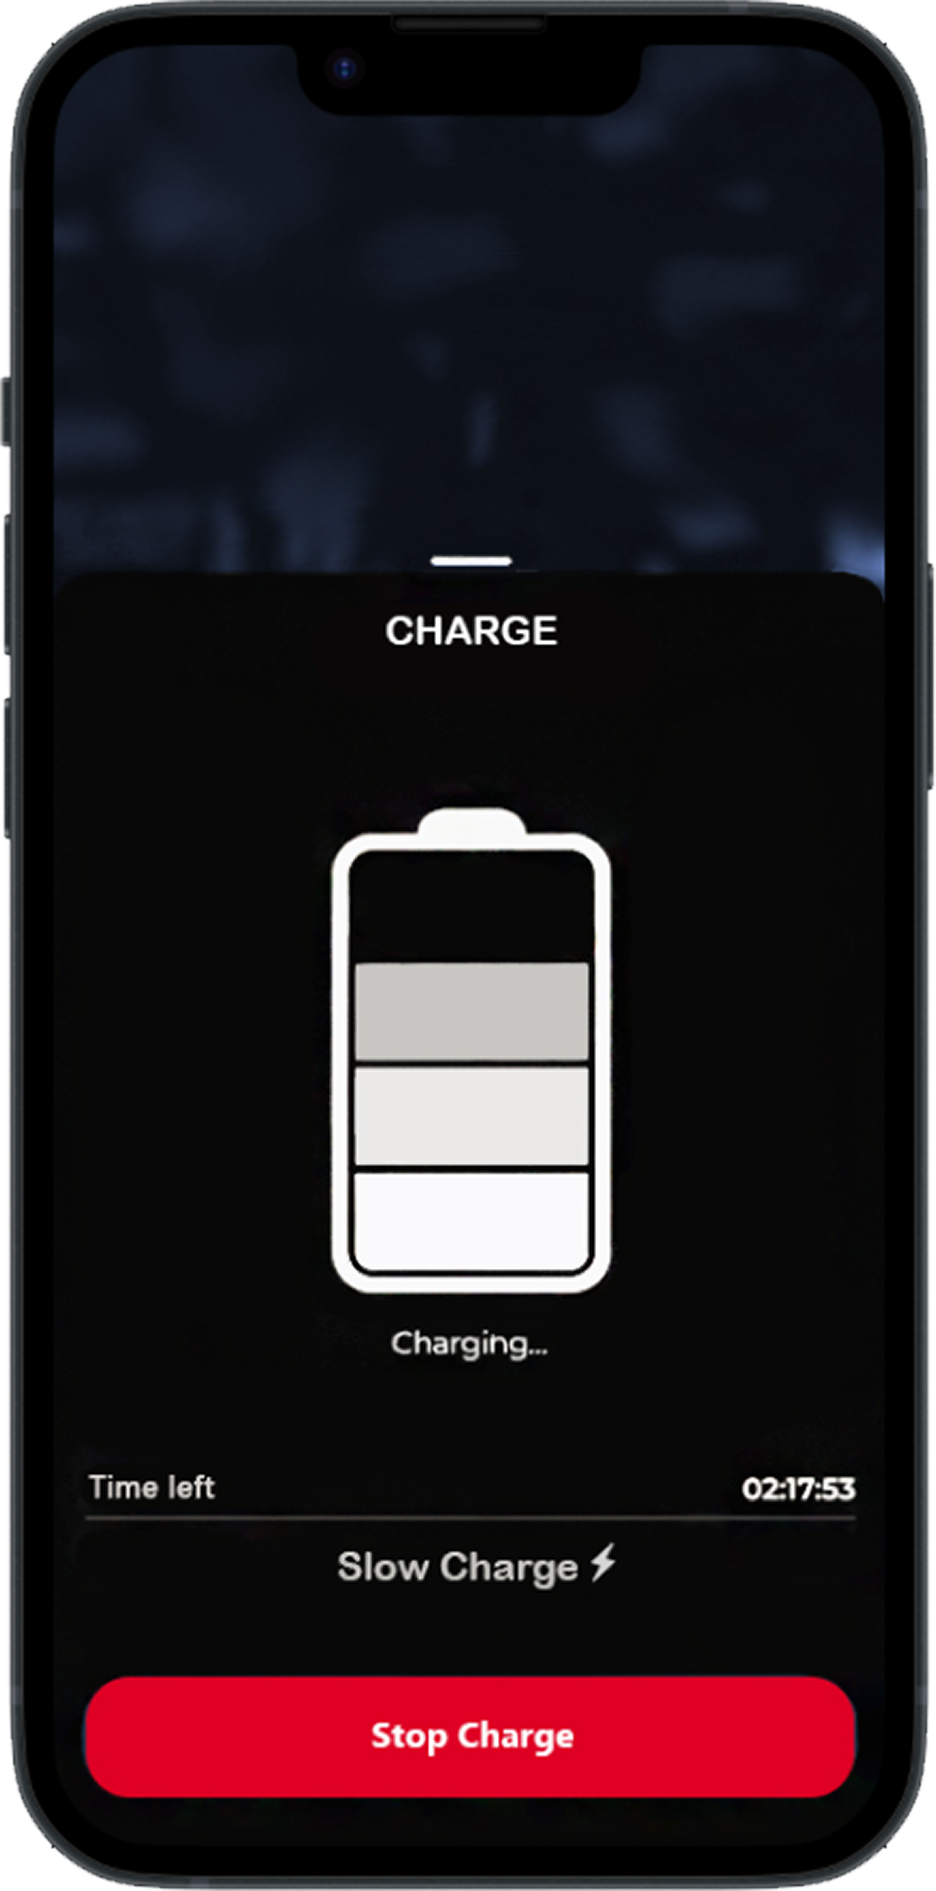
\includegraphics[width=\textwidth]{Mock/eMSP/ChargingProcess}
    \caption{Charging Process Page}
    \label{fig:ChargingProcess}
\end{minipage}
\end{figure}
The mockups depict the charging process functionality. On the left, the personal booking page (accessible from the map page) is shown, where the Driver can view their booked charge details and delete it before the arrival time. After the arrival time, the start charge button becomes active and the Driver can initiate the charging process. On the right image, the charging view is depicted, with the estimated time to complete the charge and the option to interrupt it prematurely by pressing the 'Stop Charge' button.
\end{preface}
\newpage
\section{CPMS}
\vspace{4cm}
\begin{figure}[H]
    \begin{center}
    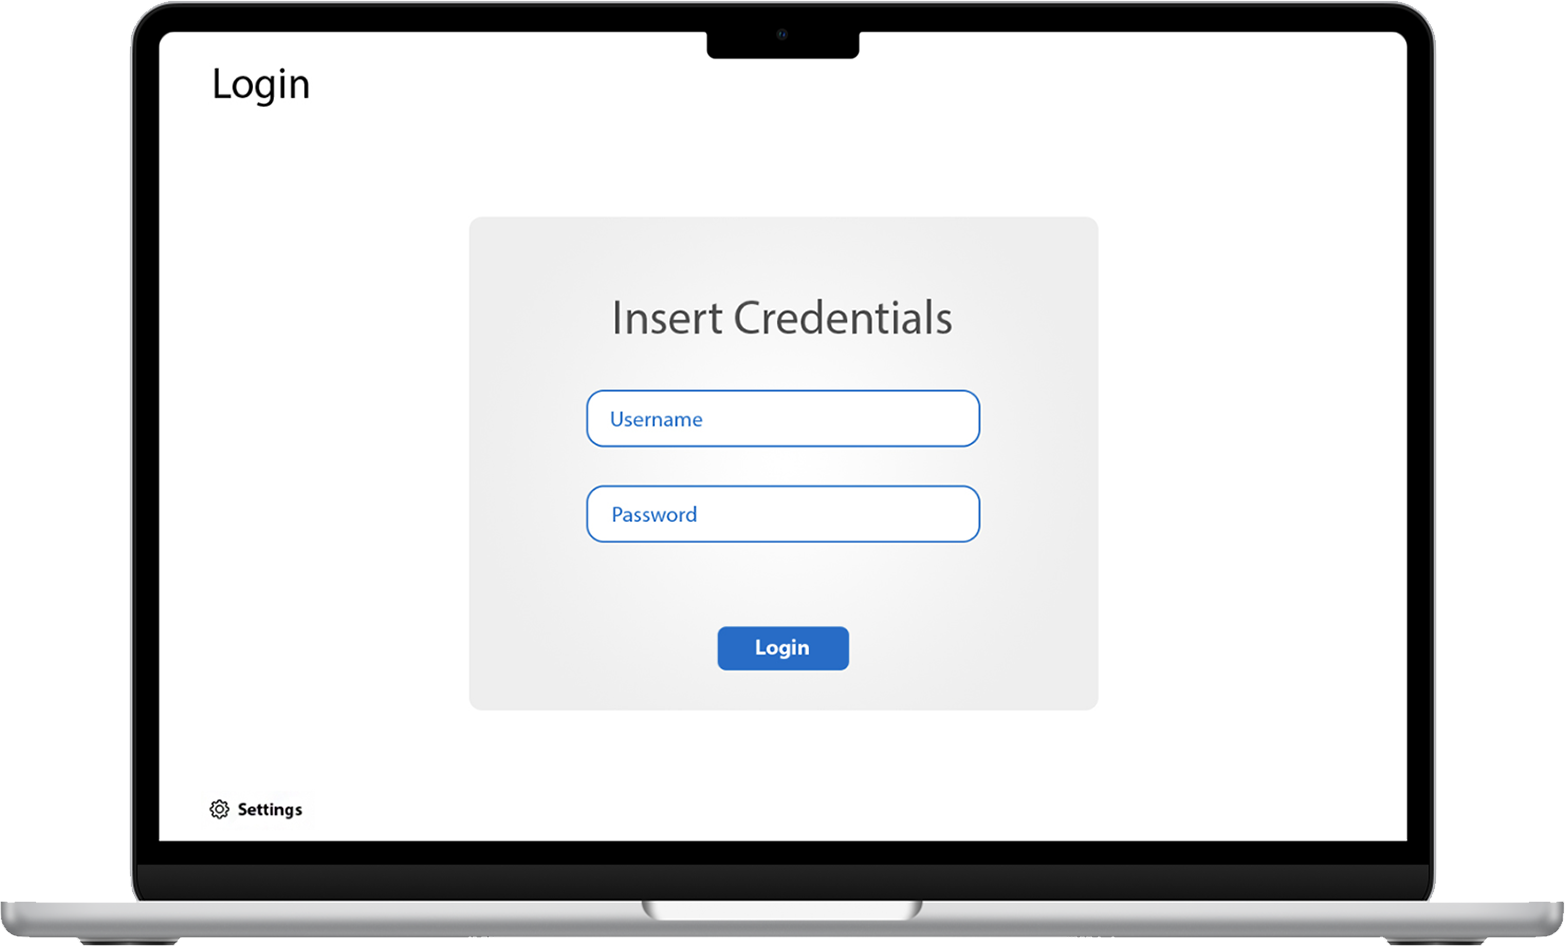
\includegraphics[
        width=\textwidth,
        height=\textheight,
        keepaspectratio]{Mock/CPMS/CPMSLogin}
    \caption{Login Page}
    \label{fig:CPMSLogin}
    \end{center}
\end{figure}
The mockup shows the login page where the CPO can access the CPMS by submitting his credentials.
\newpage
\begin{preface}
\begin{figure}[H]
    \begin{center}
    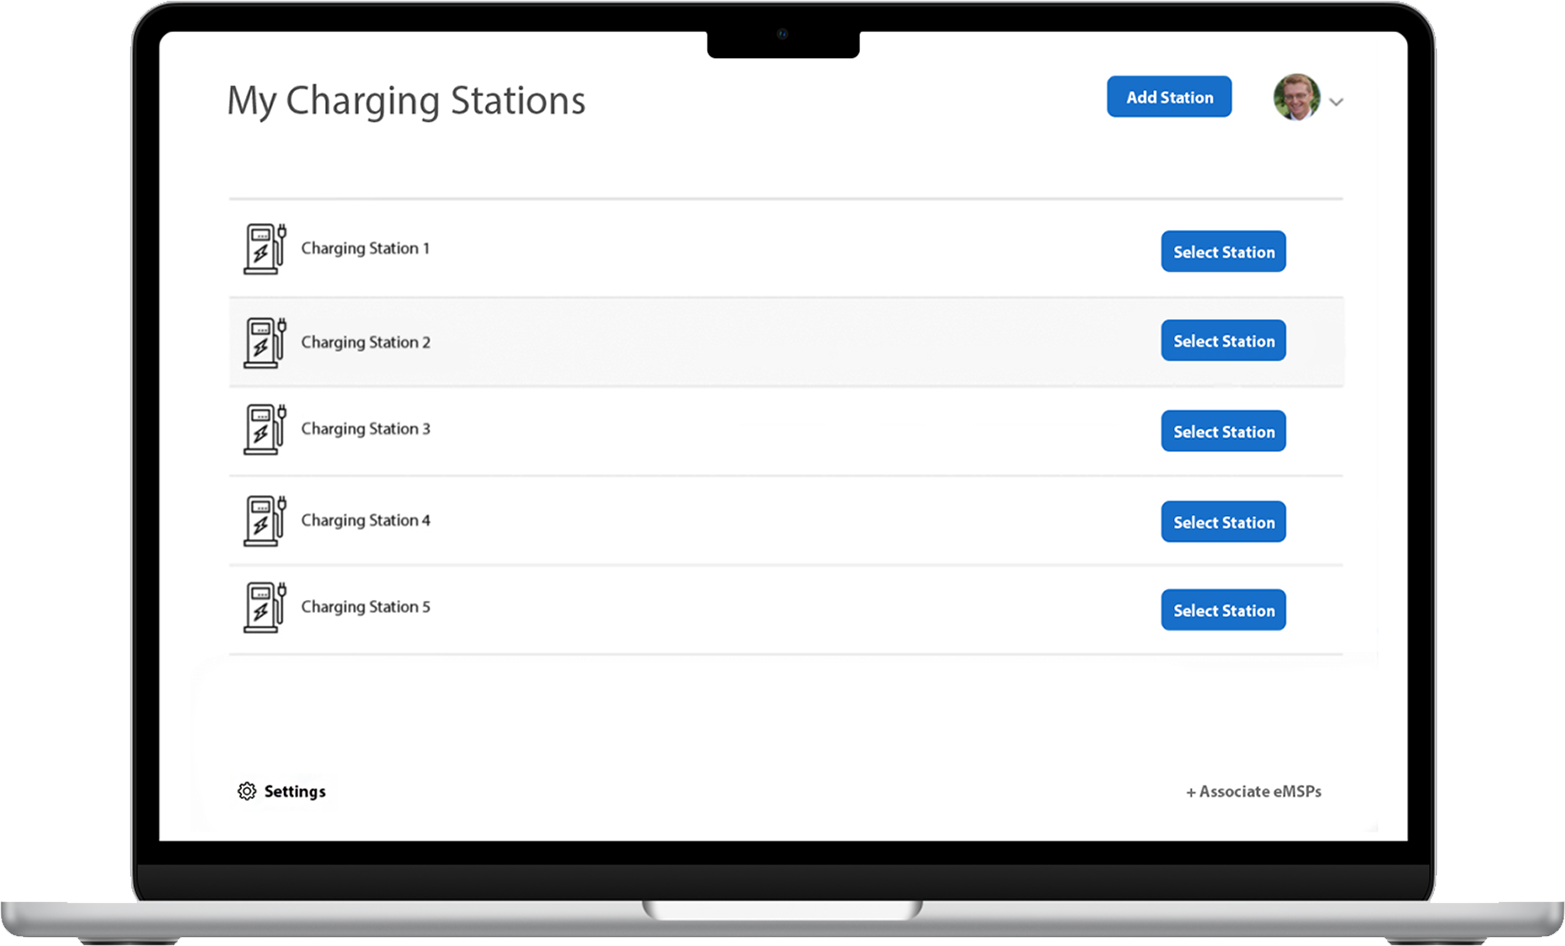
\includegraphics[
        width=\textwidth,
        height=\textheight,
        keepaspectratio]{Mock/CPMS/CPMSHome}
    \caption{Home Page}
    \label{fig:CPMSHome}
    \end{center}
\end{figure}
The mockup shows the home page of the CPMS, from which the CPO can select his managed stations to monitor them, add a new station or associate new eMSPs.
\end{preface}
\newpage
\begin{preface}
\begin{figure}[H]
    \begin{center}
    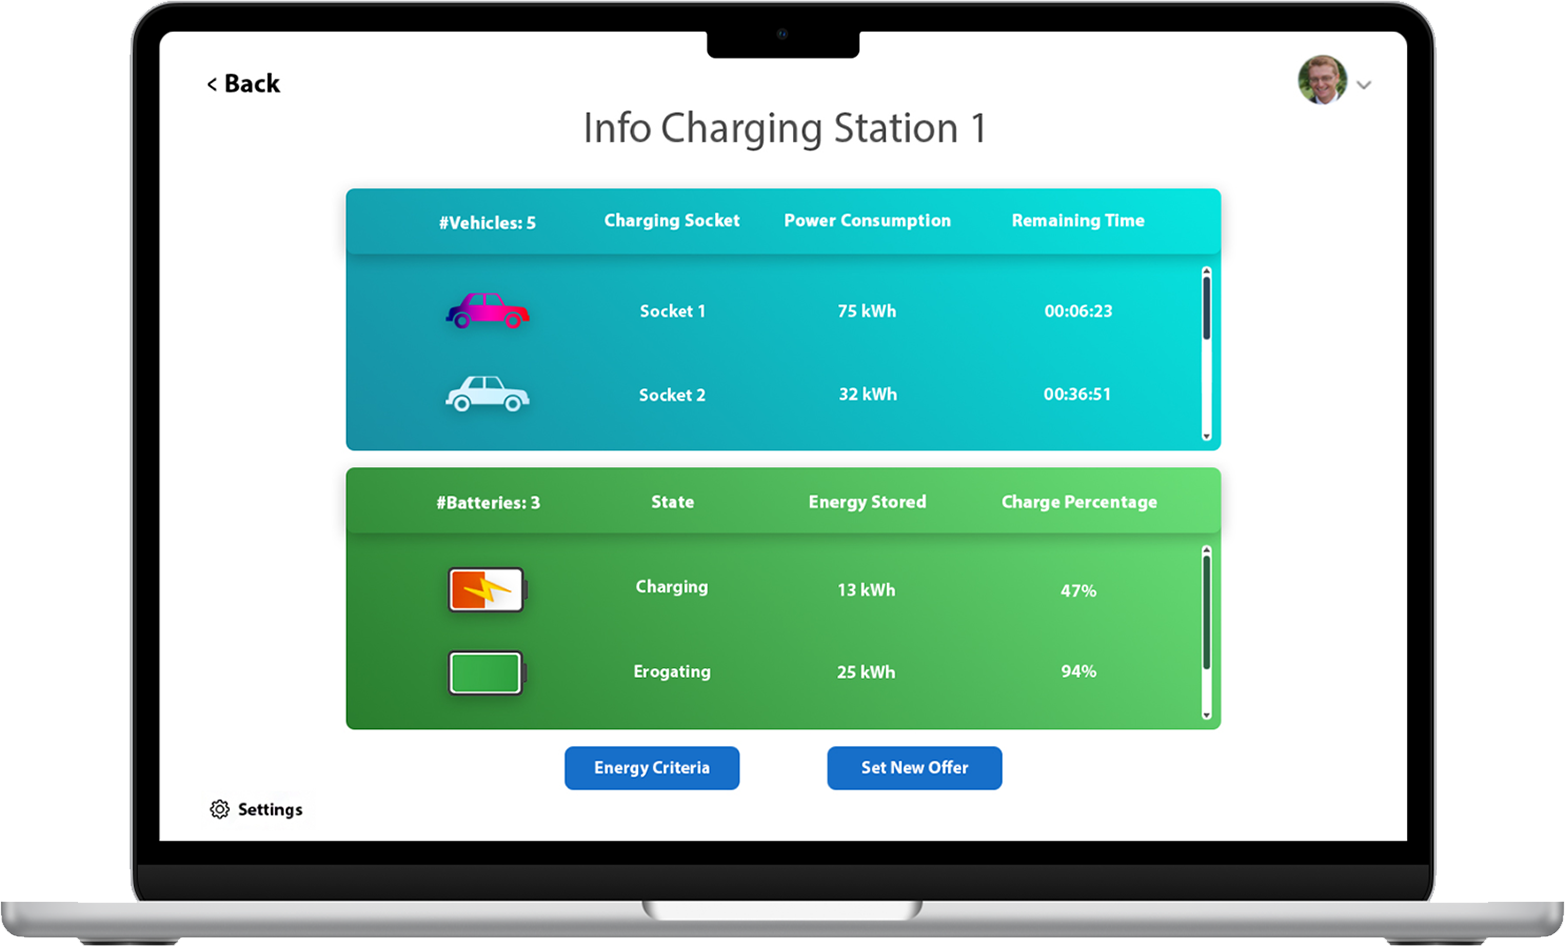
\includegraphics[
        width=\textwidth,
        height=\textheight,
        keepaspectratio]{Mock/CPMS/ChargingStationInfo}
    \caption{Charging Station Info Page}
    \label{fig:ChargingStationInfo}
    \end{center}
\end{figure}
The mockup shows an info page for a charging station, accessible from the main page. Here the CPO can see the status of the station's sockets and batteries. Also, he can update the station's energy criteria and set a new offer.
\end{preface}
\newpage
\begin{preface}
\begin{figure}[H]
    \begin{center}
    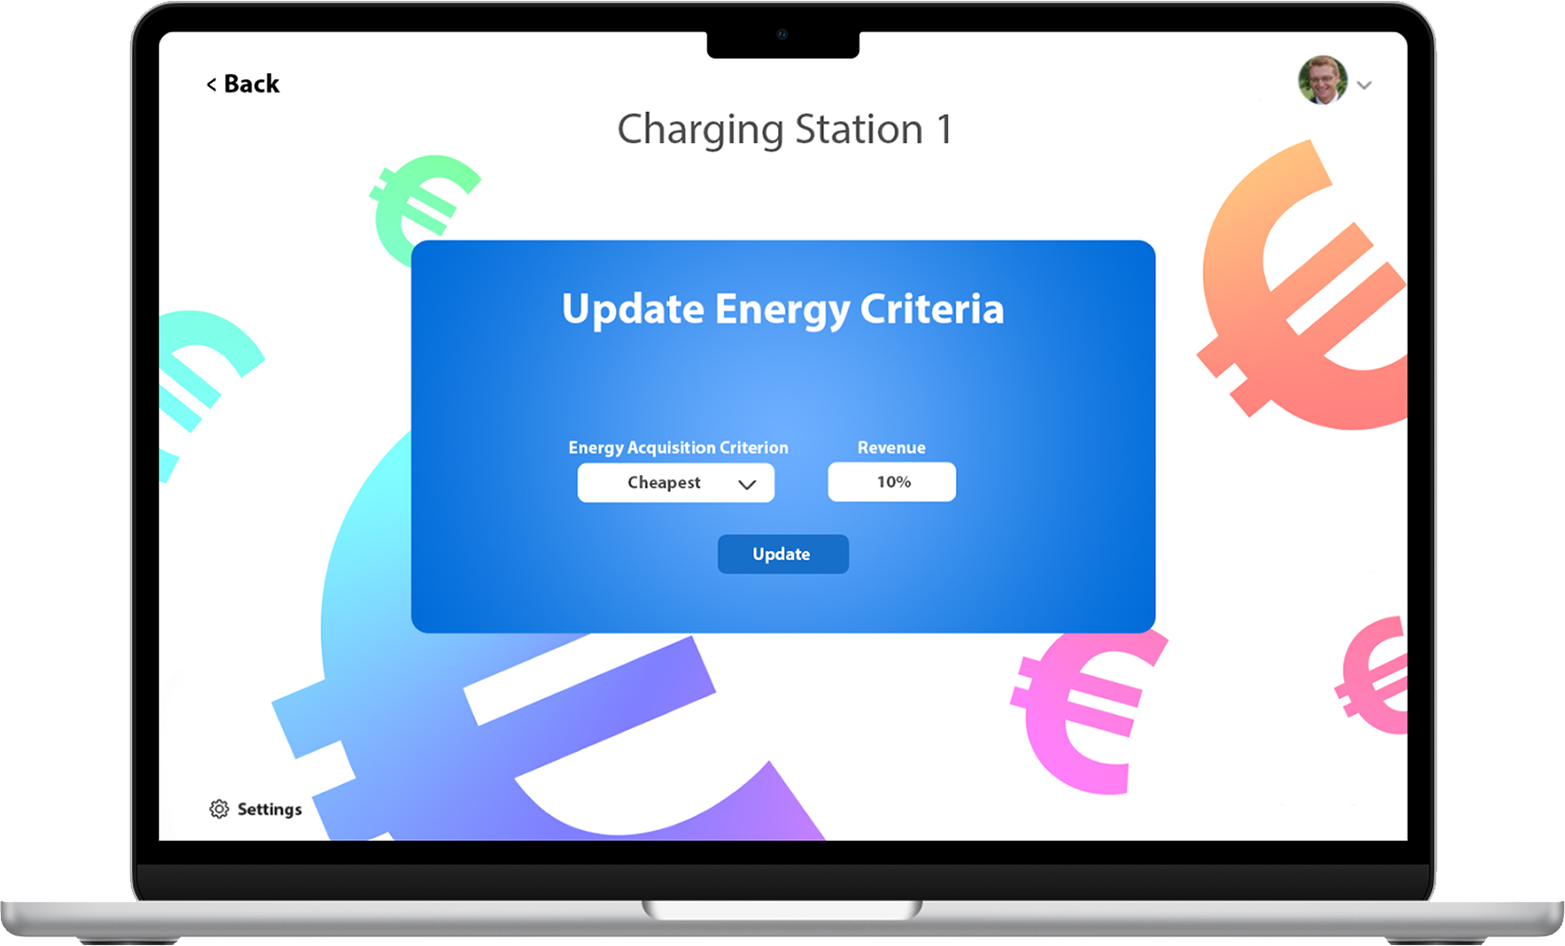
\includegraphics[
        width=\textwidth,
        height=\textheight,
        keepaspectratio]{Mock/CPMS/UpdateCriteria}
    \caption{Update Criteria Page}
    \label{fig:CPMSLogin}
    \end{center}
\end{figure}
The mockup shows the energy criteria page, accessible from the station info page, from which the CPO can update the energy acquisition criteria and the revenue for the selected charging station.
\end{preface}
\newpage
\begin{preface}
\begin{figure}[H]
    \begin{center}
    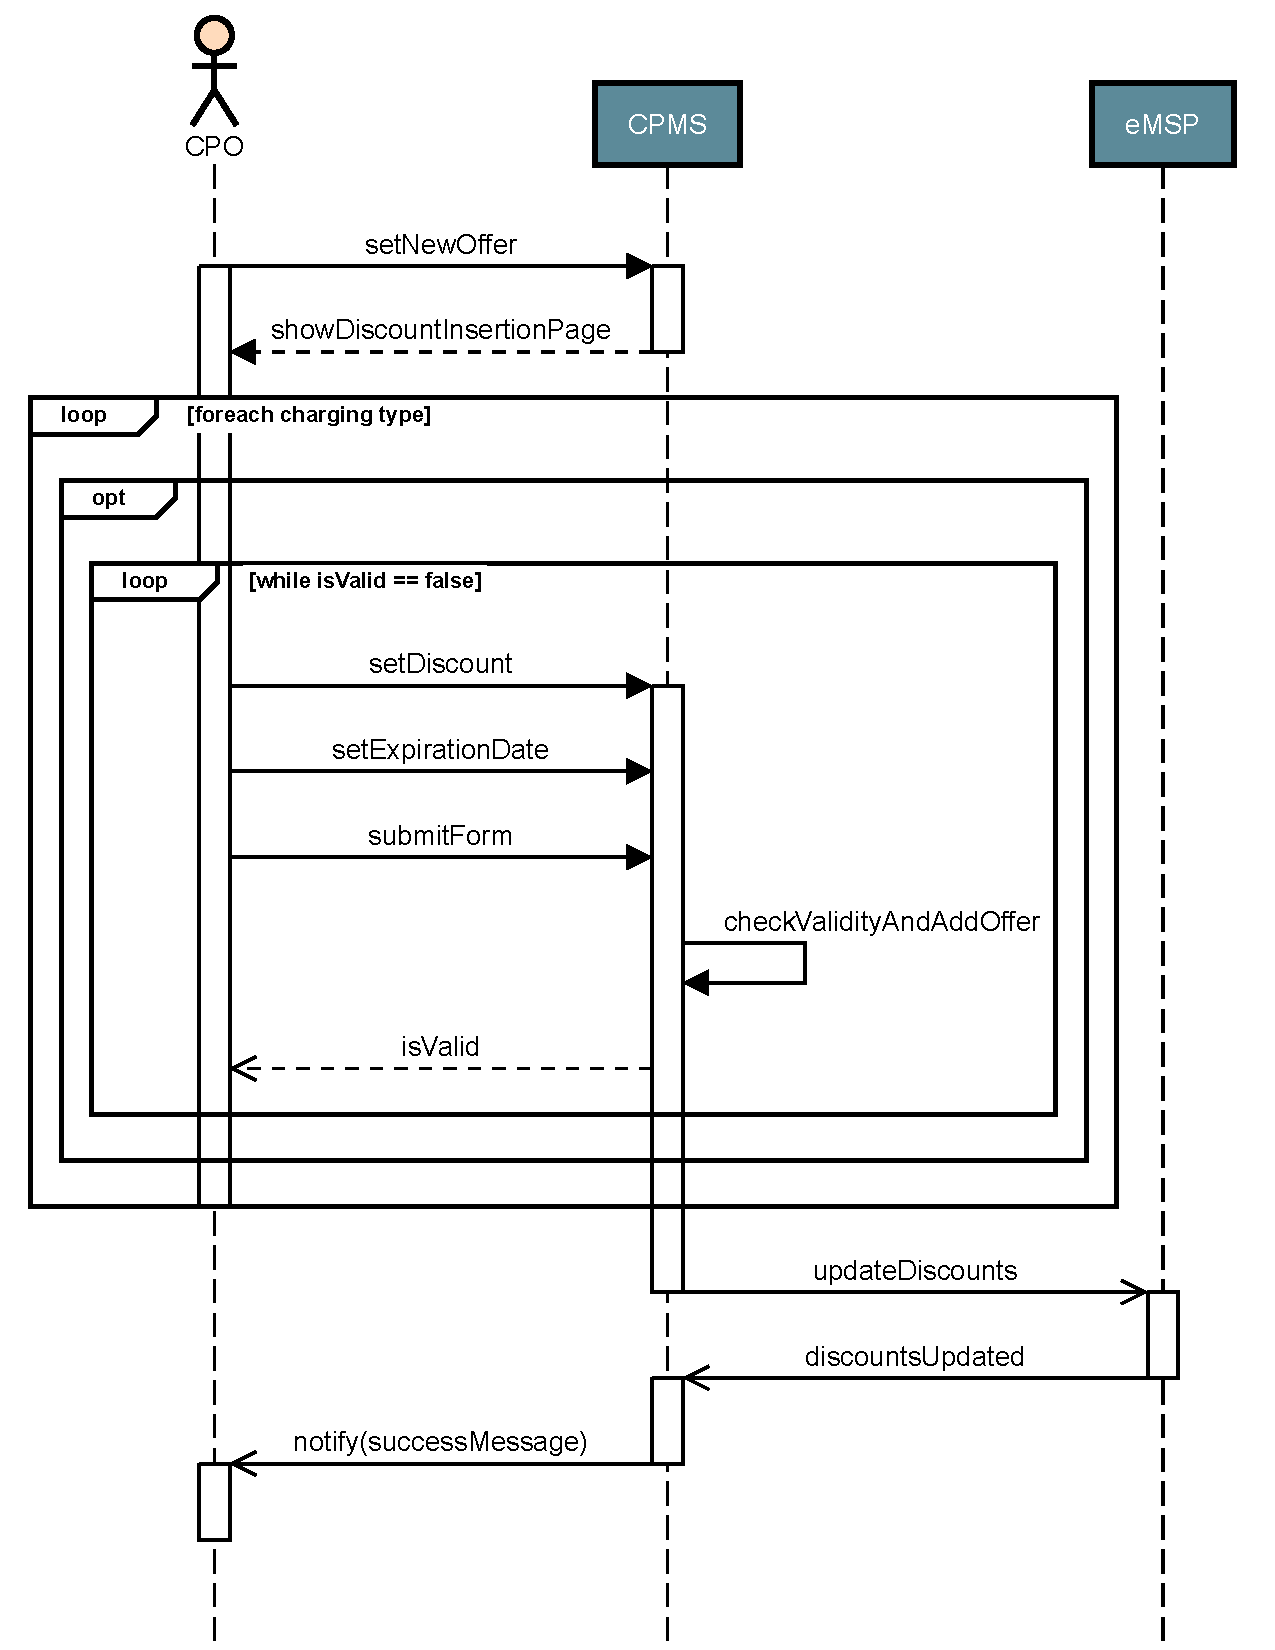
\includegraphics[
        width=\textwidth,
        height=\textheight,
        keepaspectratio]{Mock/CPMS/SetOffer}
    \caption{Set Offer Page}
    \label{fig:SetOffer}
    \end{center}
\end{figure}
The mockup shows the set offer page, accessible from the station info page, from which the CPO can set an offer for each individual charging type supported by that charging station and also insert its expiration date.
\end{preface}
\newpage
\begin{preface}
\begin{figure}[H]
    \begin{center}
    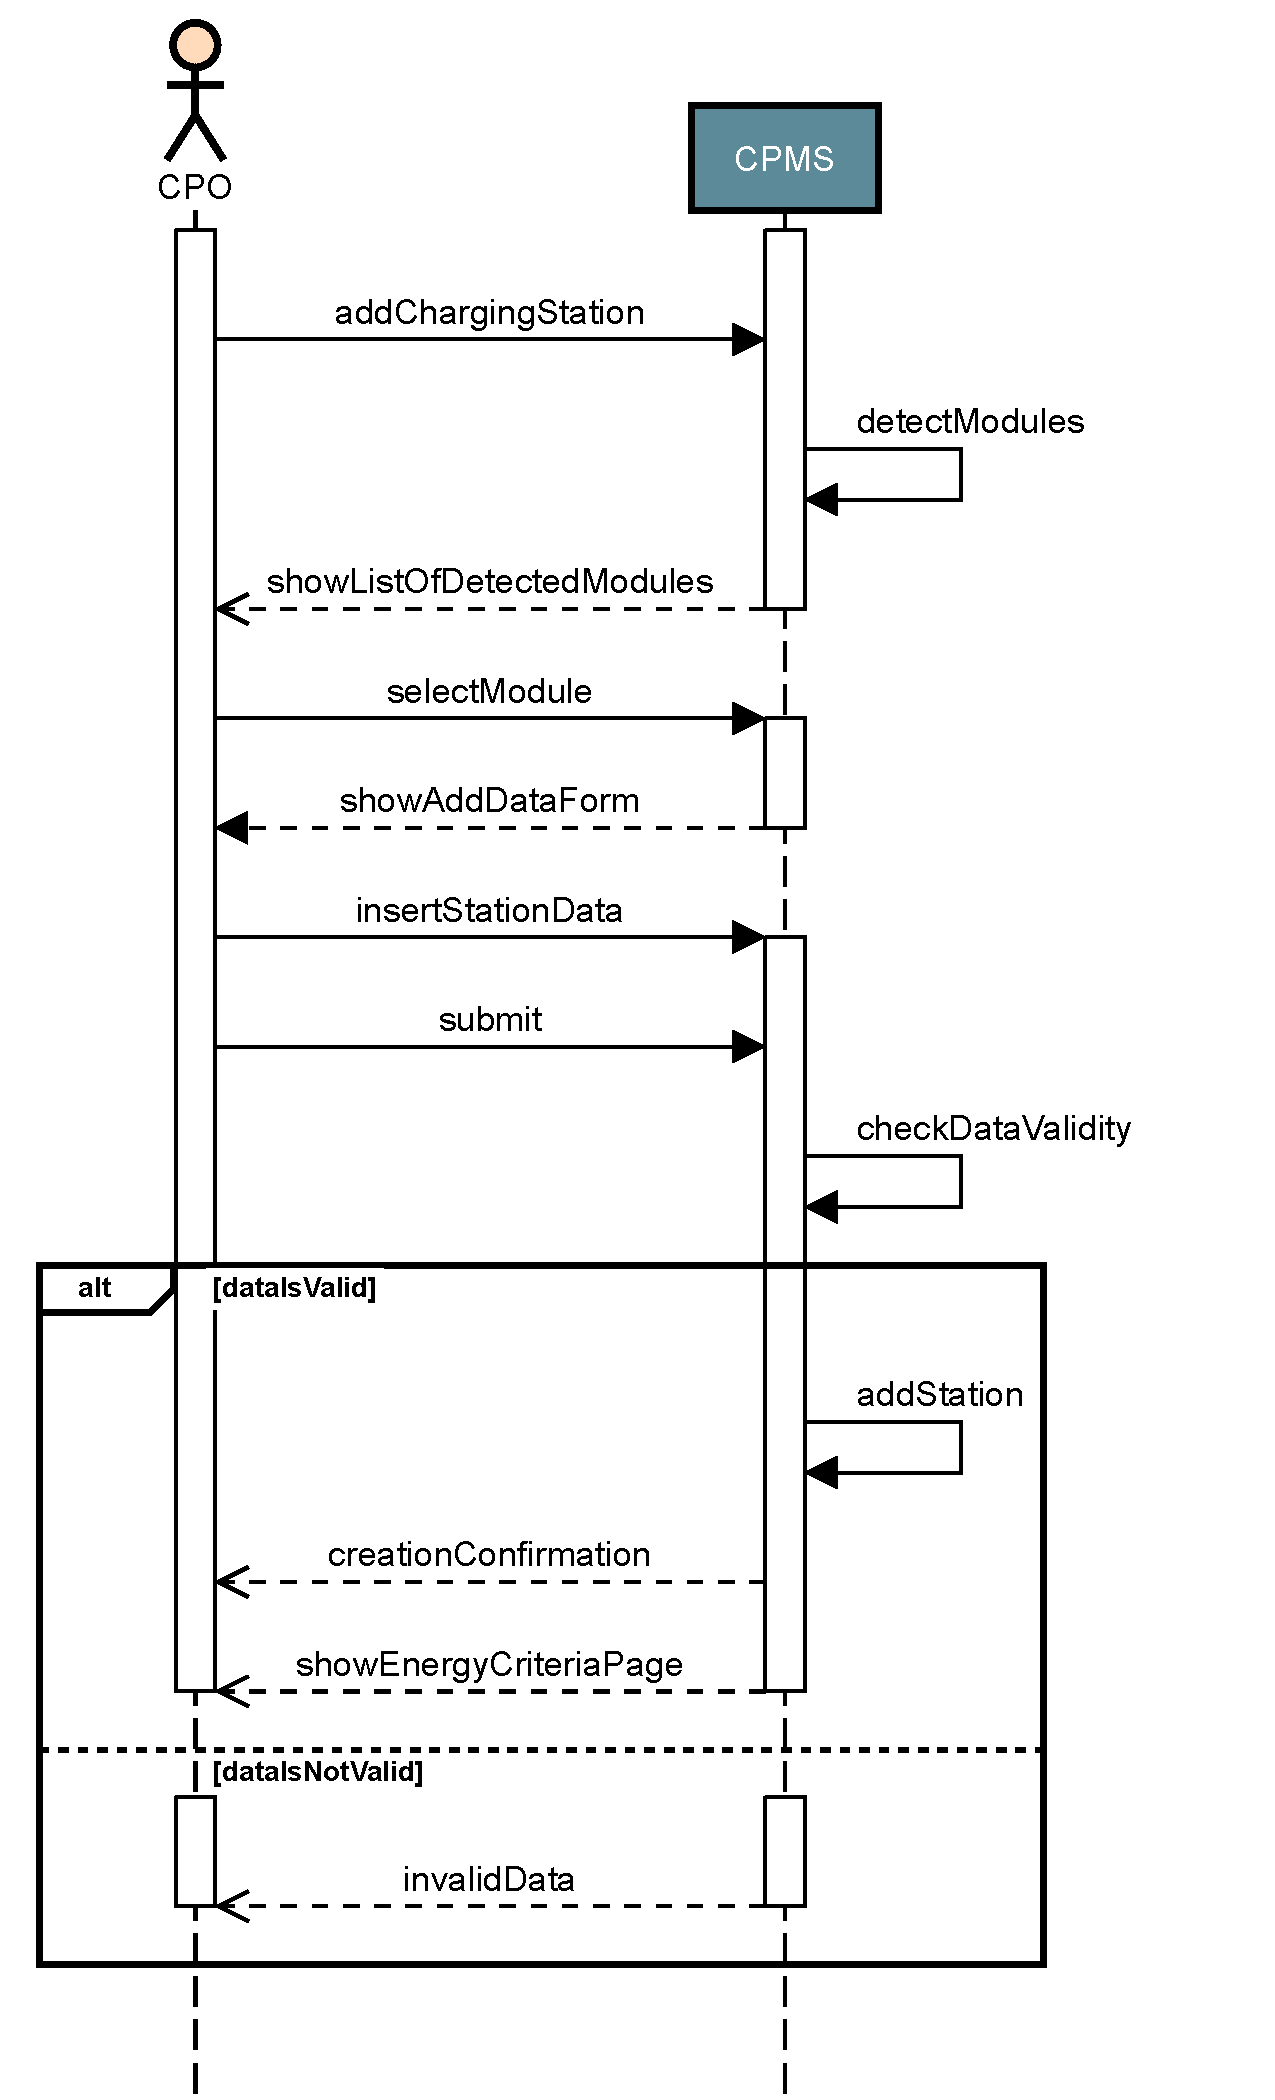
\includegraphics[
        width=\textwidth,
        height=\textheight,
        keepaspectratio]{Mock/CPMS/AddStation}
    \caption{Add Station Page}
    \label{fig:AddStation}
    \end{center}
\end{figure}
The mockup shows the add station page, accessible from the main page, from which the CPO can add a new detected charging station to the ones managed by the CPMS, inserting its name, location and supported charging types.
\end{preface}
\newpage
\begin{preface}
\begin{figure}[H]
    \begin{center}
    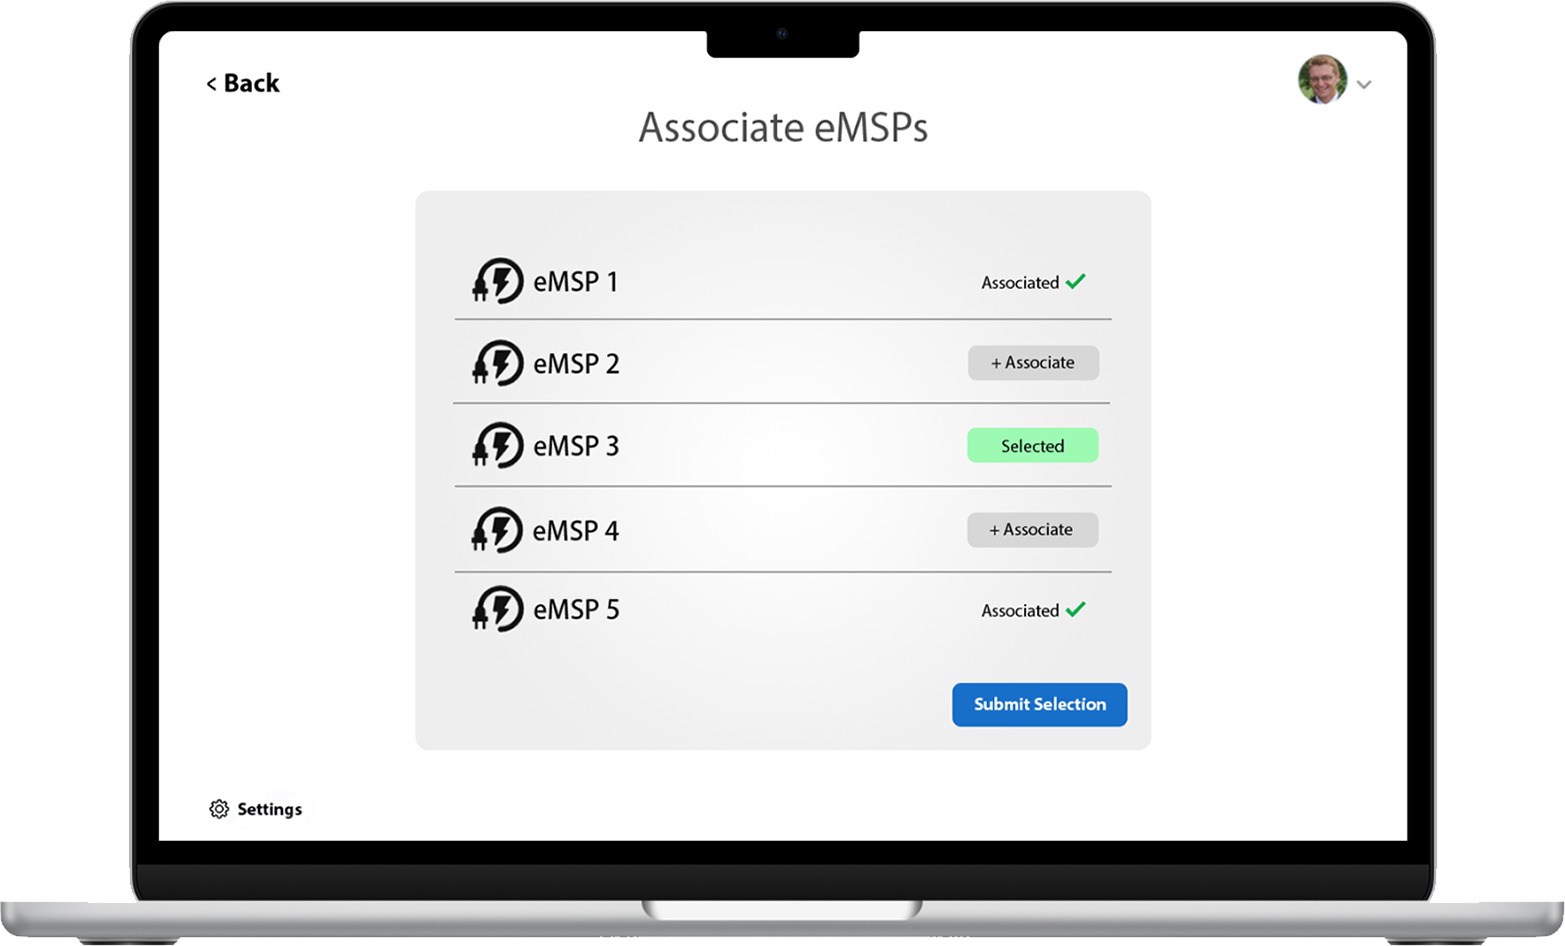
\includegraphics[
        width=\textwidth,
        height=\textheight,
        keepaspectratio]{Mock/CPMS/AssociateeMSP}
    \caption{Associate eMSPs Page}
    \label{fig:AssociateeMSP}
    \end{center}
\end{figure}
The mockup shows the eMSP association page, accessible from the main page, from which the CPO can select the eMSPs with which he wants its CPMS to associate. On the same page, he can also see the already associated ones.
\end{preface}

\restoregeometry